\documentclass[leqno]{article}
\usepackage[utf8]{inputenc}
\usepackage{enumitem}
\usepackage{tikz}
\usepackage[parfill]{parskip}
\usepackage{mathtools}
\usepackage{amsmath}
\usepackage{amssymb}

\title{Computationele logica}
\author{
    Kamans, Jim\\
    \texttt{10302905}
    \and
    Roosingh, Sander\\
    \texttt{11983957}
    \and
    Schenk, Stefan\\
    \texttt{11881798}
}
\date{December 2017}

\begin{document}

\maketitle

%%%%%%%%%%%%%%%%%%%%%%%%%%%%%%%%%%%%%%%%%%%%%%%%%%%%%%%%%%%%%%%%%%%%%%%%%%%%%%%
%% Exercise 1 %%
%%%%%%%%%%%%%%%%%%%%%%%%%%%%%%%%%%%%%%%%%%%%%%%%%%%%%%%%%%%%%%%%%%%%%%%%%%%%%%%
\section*{Exercise 1}
A robot is in a war zone. It doesn’t know its location, but all it cares is
whether or not there is a mine in front (m), and whether or not there is an
enemy approaching (e).

\begin{enumerate}
  \item \textit{Represent the robots’s belief-revision structure using a
  single-agent plausibility model, with four possible states, using the atomic
  sentences m for “there is a mine in front of the robot”, and e for “an enemy
  is approaching”.}

  \begin{center}
  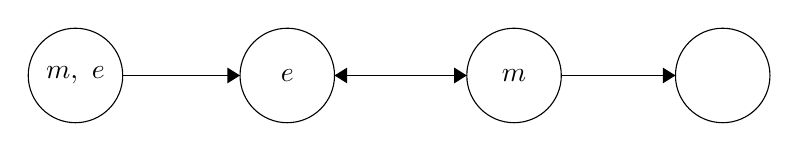
\begin{tikzpicture}[scale=0.2]
  \tikzstyle{every node}+=[inner sep=0pt]
  \draw [black] (35.95,-14.6) circle (3);
  \draw (35.95,-14.6) node {$e$};
  \draw [black] (50.35,-14.6) circle (3);
  \draw (50.35,-14.6) node {$m$};
  \draw [black] (63.6,-14.6) circle (3);
  \draw [black] (22.5,-14.6) circle (3);
  \draw (22.5,-14.6) node {$m,\mbox{ }e$};
  \draw [black] (38.95,-14.6) -- (47.35,-14.6);
  \fill [black] (47.35,-14.6) -- (46.55,-14.1) -- (46.55,-15.1);
  \draw [black] (47.35,-14.6) -- (38.95,-14.6);
  \fill [black] (38.95,-14.6) -- (39.75,-15.1) -- (39.75,-14.1);
  \draw [black] (25.5,-14.6) -- (32.95,-14.6);
  \fill [black] (32.95,-14.6) -- (32.15,-14.1) -- (32.15,-15.1);
  \draw [black] (53.35,-14.6) -- (60.6,-14.6);
  \fill [black] (60.6,-14.6) -- (59.8,-14.1) -- (59.8,-15.1);
  \end{tikzpicture}
  \end{center}

  \item \textit{Suppose now that the robot’s sensors indicate some vibrations.}

  \begin{center}
  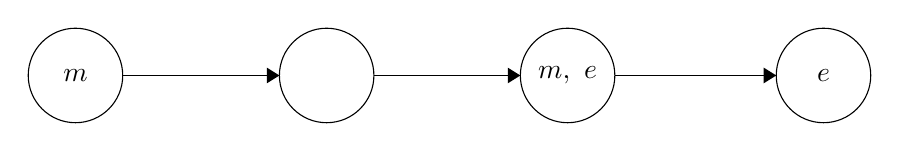
\begin{tikzpicture}[scale=0.2]
  \tikzstyle{every node}+=[inner sep=0pt]
  \draw [black] (65.45,-11.7) circle (3);
  \draw (65.45,-11.7) node {$e$};
  \draw [black] (17.95,-11.7) circle (3);
  \draw (17.95,-11.7) node {$m$};
  \draw [black] (33.9,-11.7) circle (3);
  \draw [black] (49.2,-11.7) circle (3);
  \draw (49.2,-11.7) node {$m,\mbox{ }e$};
  \draw [black] (20.95,-11.7) -- (30.9,-11.7);
  \fill [black] (30.9,-11.7) -- (30.1,-11.2) -- (30.1,-12.2);
  \draw [black] (36.9,-11.7) -- (46.2,-11.7);
  \fill [black] (46.2,-11.7) -- (45.4,-11.2) -- (45.4,-12.2);
  \draw [black] (52.2,-11.7) -- (62.45,-11.7);
  \fill [black] (62.45,-11.7) -- (61.65,-11.2) -- (61.65,-12.2);
  \end{tikzpicture}
  \end{center}

  \item \textit{Immediately after the event in the previous part, the robot’s metal detector indicates the presence of a mine}

  \begin{center}
  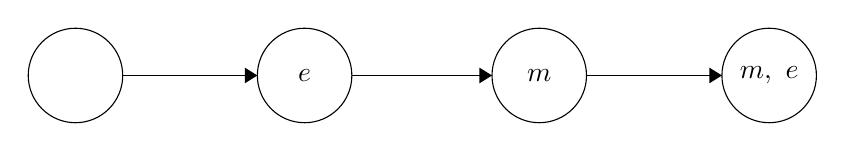
\begin{tikzpicture}[scale=0.2]
  \tikzstyle{every node}+=[inner sep=0pt]
  \draw [black] (35.95,-22.9) circle (3);
  \draw (35.95,-22.9) node {$e$};
  \draw [black] (50.85,-22.9) circle (3);
  \draw (50.85,-22.9) node {$m$};
  \draw [black] (21.4,-22.9) circle (3);
  \draw [black] (65.45,-22.9) circle (3);
  \draw (65.45,-22.9) node {$m,\mbox{ }e$};
  \draw [black] (24.4,-22.9) -- (32.95,-22.9);
  \fill [black] (32.95,-22.9) -- (32.15,-22.4) -- (32.15,-23.4);
  \draw [black] (38.95,-22.9) -- (47.85,-22.9);
  \fill [black] (47.85,-22.9) -- (47.05,-22.4) -- (47.05,-23.4);
  \draw [black] (53.85,-22.9) -- (62.45,-22.9);
  \fill [black] (62.45,-22.9) -- (61.65,-22.4) -- (61.65,-23.4);
  \end{tikzpicture}
  \end{center}

  \item \textit{}

	\item \textit{Represent the robot's belief-revision structure using a single-agent plausibility model,} with four possible states, using the atomic sentences $m$ for "there is a mine in front of the robot", and $e$ for "an enemy is approaching". Draw arrows going from the less plausible worlds to more plausible worlds (according to the robot's plausibility relation). In your drawing, you may skip the loops (since plausibility relations are assumed to be reflexive) and the arrows that can be obtained by composing other arrows (since plausibility relations are assumed to be transitive), but be aware that they are there. Also, be sure to use all information given in the text above.\\
	\begin{center}
		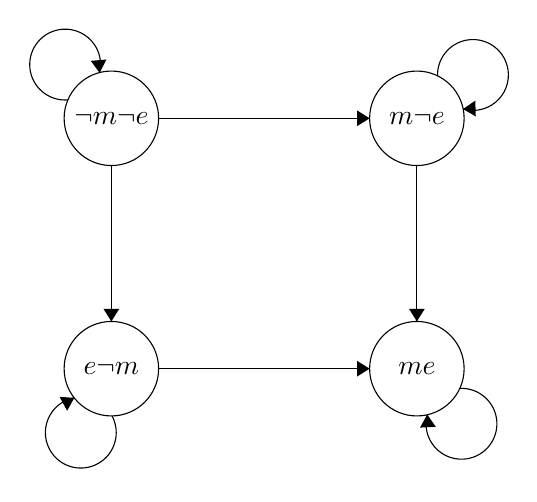
\begin{tikzpicture}[scale=0.2]
		\tikzstyle{every node}+=[inner sep=0pt]
		\draw [black] (46.3,-17) circle (3);
		\draw (46.3,-17) node {$m \neg e$};
		\draw [black] (26.9,-32.9) circle (3);
		\draw (26.9,-32.9) node {$e \neg m$};
		\draw [black] (26.9,-17) circle (3);
		\draw (26.9,-17) node {$\neg m \neg e$};
		\draw [black] (46.3,-32.9) circle (3);
		\draw (46.3,-32.9) node {$me$};
		\draw [black] (26.9,-20) -- (26.9,-29.9);
		\fill [black] (26.9,-29.9) -- (27.4,-29.1) -- (26.4,-29.1);
		\draw [black] (29.9,-32.9) -- (43.3,-32.9);
		\fill [black] (43.3,-32.9) -- (42.5,-32.4) -- (42.5,-33.4);
		\draw [black] (46.3,-20) -- (46.3,-29.9);
		\fill [black] (46.3,-29.9) -- (46.8,-29.1) -- (45.8,-29.1);
		\draw [black] (29.9,-17) -- (43.3,-17);
		\fill [black] (43.3,-17) -- (42.5,-16.5) -- (42.5,-17.5);
		\draw [black] (47.612,-14.315) arc (181.69424:-106.30576:2.25);
		\fill [black] (49.23,-16.41) -- (50.04,-16.88) -- (50.01,-15.88);
		\draw [black] (24.15,-15.831) arc (274.71268:-13.28732:2.25);
		\fill [black] (26.15,-14.11) -- (26.59,-13.27) -- (25.59,-13.35);
		\draw [black] (26.937,-35.888) arc (28.44003:-259.55997:2.25);
		\fill [black] (24.55,-34.75) -- (23.61,-34.69) -- (24.09,-35.57);
		\draw [black] (49.014,-34.151) arc (92.99099:-195.00901:2.25);
		\fill [black] (46.96,-35.81) -- (46.5,-36.64) -- (47.5,-36.59);
		\end{tikzpicture}
	\end{center}

	\item
	\item
	\item
	\item
	\item
\end{enumerate}

%%%%%%%%%%%%%%%%%%%%%%%%%%%%%%%%%%%%%%%%%%%%%%%%%%%%%%%%%%%%%%%%%%%%%%%%%%%%%%%
%% Exercise 2 %%
%%%%%%%%%%%%%%%%%%%%%%%%%%%%%%%%%%%%%%%%%%%%%%%%%%%%%%%%%%%%%%%%%%%%%%%%%%%%%%%
\section*{Exercise 2}
\begin{enumerate}

	\item

	\item

	\item

	\item

	\item

\end{enumerate}

\end{document}
